
\begin{enumerate}
\item {\color{red}\textit{¿Pueden  los protocolos de enrutamiento estáticos y dinámicos trabajar al mismo tiempo en una tabla del router?}}\\
Sí, es posible que se apliquen enrutamiento estático y dinámico al mismo tiempo; el router tendrá preferencia hacia rutas estáticas de la misma longitud que las del proceso de enrutamiento, siempre que no se aplique ninguna manipulación manual de la ruta.\cite{routing6}. En el caso de trabajar \textbf{en una misma tabla}
no se podría porque el dinamico actualizaría los datos y dejaría de ser estático.
\item {\color{red}\textit{¿Pueden estar habilitados más de un protocolo dinámico en un mismo  router?}}\\
Sí, se puede ejecutar varios protocolos de enrutamiento para llegar al mismo destino. Pero la ruta aprendida mediante el protocolo de enrutamiento con la métrica/distancia administrativa (AD) más baja se considerará como la mejor ruta.
\item {\color{red}\textit{¿Si ud. es un administrador de una red de un Banco, que protocolos de enrutamiento utilizaría en su red? ¿Porque?}}

Basado en estas respuestas encontré \cite{protos}\cite{protos2} que  los protocolos de enrutamiento utilizados vendrían determinados por los dispositivos de red utilizados y el diseño general de la red. EIGRP parece el mas utilizado en redes con dispositivos Cisco o de terceros que soporten este método esto debido a que EIGRP utiliza RTP en lugar de UDP o TCP, o bien OGRP en el caso de dispositivos de multiples fabricantes.

\item {\color{red}\textit{¿Como son consideradas las rutas que son ingresadas de manera estática vs. los que son ingresados de manera dinámica? ¿Las rutas de que protocolos tiene más prioridad ?}}

Para esta pregunta existe el concepto de Distancia Administrativa
(AD: Administrative Distance) que es un valor que utilizan los routers para seleccionar la mejor ruta cuando hay dos o más rutas diferentes al mismo destino desde dos protocolos de enrutamiento diferentes.\cite{routing3} Dicho esto las rutas estáticas son las que usualmente (en algunos casos puede variar \cite{routing4}) tienen mayor prioridad esto debido a que no está aprendiendo ninguna ruta de ningún otro router a través de la red, por lo que no hay posibilidad de que el router aprenda una ruta incorrecta o no segura.\cite{routing2} \textbf{(Tabla de Prioridad en la siguiente página.)}




\item {\color{red}\textit{¿Cuales son las técnicas utilizadas por los Switches Ethernet para despachar los paquetes ethernet?}}

\begin{itemize}
\item \textbf{Aprendizaje de direcciones (Address Learning):} Como todas las interfaces Ethernet, cada puerto de un switch tiene una dirección MAC exclusiva asignada de fábrica. Sin embargo, a diferencia de un dispositivo Ethernet normal que acepta solo tramas dirigidas a él, la interfaz Ethernet ubicada en cada puerto de un switch se ejecuta en modo promiscuo. En este modo, la interfaz está programada para recibir todas las tramas que ve en ese puerto, no solo las tramas que se envían a la dirección MAC de la interfaz Ethernet en ese puerto de conmutador. A medida que se recibe cada trama en cada puerto, el software de conmutación observa la dirección de origen de la trama y agrega esa dirección de origen a una tabla de direcciones que mantiene el switch. Así es como el switch descubre automáticamente qué estaciones son accesibles en qué puertos.
\item \textbf{Filtrado de Tráfico (Traffic Filtering):} El switch tiene la capacidad de almacenar tramas en la memoria antes de transmitirlas al cable Ethernet conectado al puerto. Por ejemplo, si el puerto ya está ocupado transmitiendo cuando llega una trama para su transmisión, entonces la trama se puede retener durante el breve tiempo que tarda el puerto en completar la transmisión de la trama anterior. Para transmitir la trama, el conmutador coloca la trama en la cola de conmutación de paquetes para su transmisión en el otro puerto. Esto evita el flujo de tráfico innecesario en otros segmentos del sistema de red, que es una de las principales ventajas de un switch.
\item \textbf{Inundación de Tramas (Frame Flooding):} El switch reenvía la trama destinada a una estación desconocida a todos los puertos del conmutador distintos al que se recibió, inundando así la trama a todas las demás estaciones. Inundar la trama garantiza que una trama con una dirección de destino desconocida llegará a todas las conexiones de red y será escuchada por el dispositivo de destino correcto, asumiendo que está activo y en la red. Cuando el dispositivo desconocido responde con tráfico de retorno, el switch aprenderá automáticamente en qué puerto se encuentra el dispositivo y ya no inundará el tráfico destinado a ese dispositivo.
\end{itemize}

\begin{figure}[ht!]
\centering
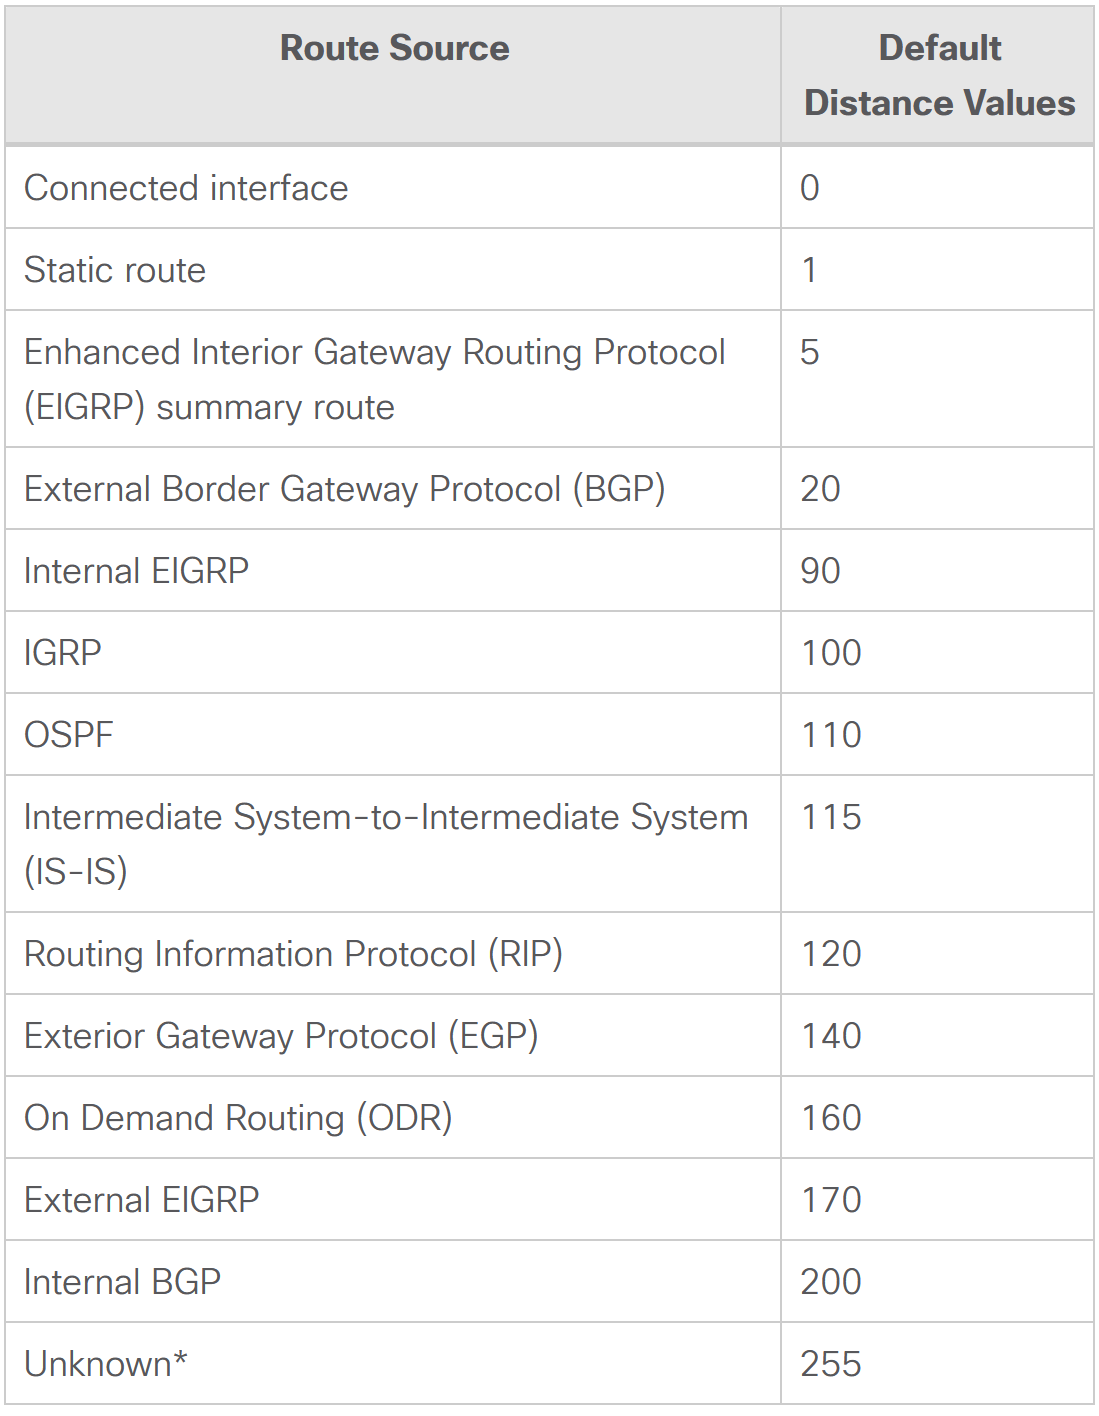
\includegraphics[scale=0.5]{Imagenes/cisco_ad.png}
\caption{What Is Administrative Distance? Cisco\cite{routing5}}
\end{figure}

\item {\color{red}\textit{En un switch con velocidad de puertos 10/100/1000, ¿Todas las maquinas deben ser de la misma velocidad? Explicar}}\\
No necesariamente, el único inconveniente es que cuando una maquina que envie muchas tramas a una de menor capacidad, el switch tiene que almacenar la trama en búfer hasta que la PC más lenta pueda recibirla. Los switches, especialmente los económicos, no tienen mucha memoria de búfer, por lo que puede terminar con frames descartados, provocando retransmisiones.

\item {\color{red}\textit{¿Cual es la diferencia entre un switch administrable y uno no administrable? ¿Cuáles son las similitudes?}}

\begin{itemize}
\item \textbf{Switch no Administrable:} Un Switch no Administrable cumple la función básica del switch en sí, lo que significa que es un dispositivo de tipo plug-and-play, se conecta a la alimentación eléctrica, se conecta a los diferentes equipos vía cable, y automáticamente se podrán comunicar entre ellos y transferir datos. 
\item \textbf{Switch Administrable:} Un switch administrable  permite administrar, configurar y monitorear la configuración de la red, incluidos los controles sobre el tráfico de la LAN, priorizando ciertos canales.
\end{itemize}


\textbf{Rendimiento} \\
La ventaja de los switches no administrables en lo que respecta al rendimiento es que puede conectarse y usar inmediatamente con su red (\textit{plug $\&$ play}). No es necesario configurar nada y tiene servicios de QoS integrados para garantizar que funcione correctamente. Sin embargo, con un switch administrable, se puede priorizar canales, lo que garantiza que obtenga el mejor rendimiento donde se necesite.\\{ }\\
\textbf{Seguridad} \\
Los switches no administrables, en general, tienen una seguridad muy básica. Están protegidos al garantizar que no tenga vulnerabilidades de un sistema a otro, de una manera en la que cosas como una cubierta de puerto con cerradura, pueden garantizar que nadie manipule el dispositivo directamente. Los switches administrables tienen algunos beneficios de seguridad importantes, como la capacidad de monitorear y controlar la red para apagar amenazas activas y protección de datos. Las características de seguridad difieren entre diferentes switches administrables.\\{ }\\
\textbf{Aplicaciones:} \\
Cuando se trata de redes más pequeñas, como las de pequeñas empresas, el hogar, una sola oficina, etc., es más probable que se utilice un switch no administrable. Los switches administrables se adaptan mejor a las empresas con un alcance de red mucho mayor, o para aquellas que usan centros de datos de cosas y necesitan un control mucho mejor sobre el tráfico dentro de su red.

\item {\color{red}\textit{¿Cuales son los comandos más comunes del IOS de los switches ?}} \\

\texttt{
Changing the hostname of a switch:\\ 
switch(config)\# hostname <name> \\
}

\texttt{
To add a banner message: \\
switch(config)\# banner motd \& \\
Enter Text message. End with character '\&' \\
\$ Confusion of da highest orda \& \\
}

\texttt{
To set IP address in Switch: \\
switch(config)\# interface vlan1 \\
switch(config-if)\# ip address 172.16.10.1 255.255.255.0 \\
switch(config-if)\# exit \\
switch(config)\# ip default-gateway 172.16.10.0 \\
}

\texttt{
To set the current clock time: \\
switch\# clock set 3:03:14 June 25 2020}

\texttt{
Enable password :\\
(config)\# enable password GFGGFG
}

\texttt{
Copy to startup-configuration file from running-configuration file :\\
switch\# copy running-config startup-config
}

\texttt{
Clear mac address table: \\
switch\# clear mac address-table
}
 
\item {\color{red}\textit{¿Cuales son los comandos más usuales del IOS para un router ?}}
\end{enumerate}
\begin{center}
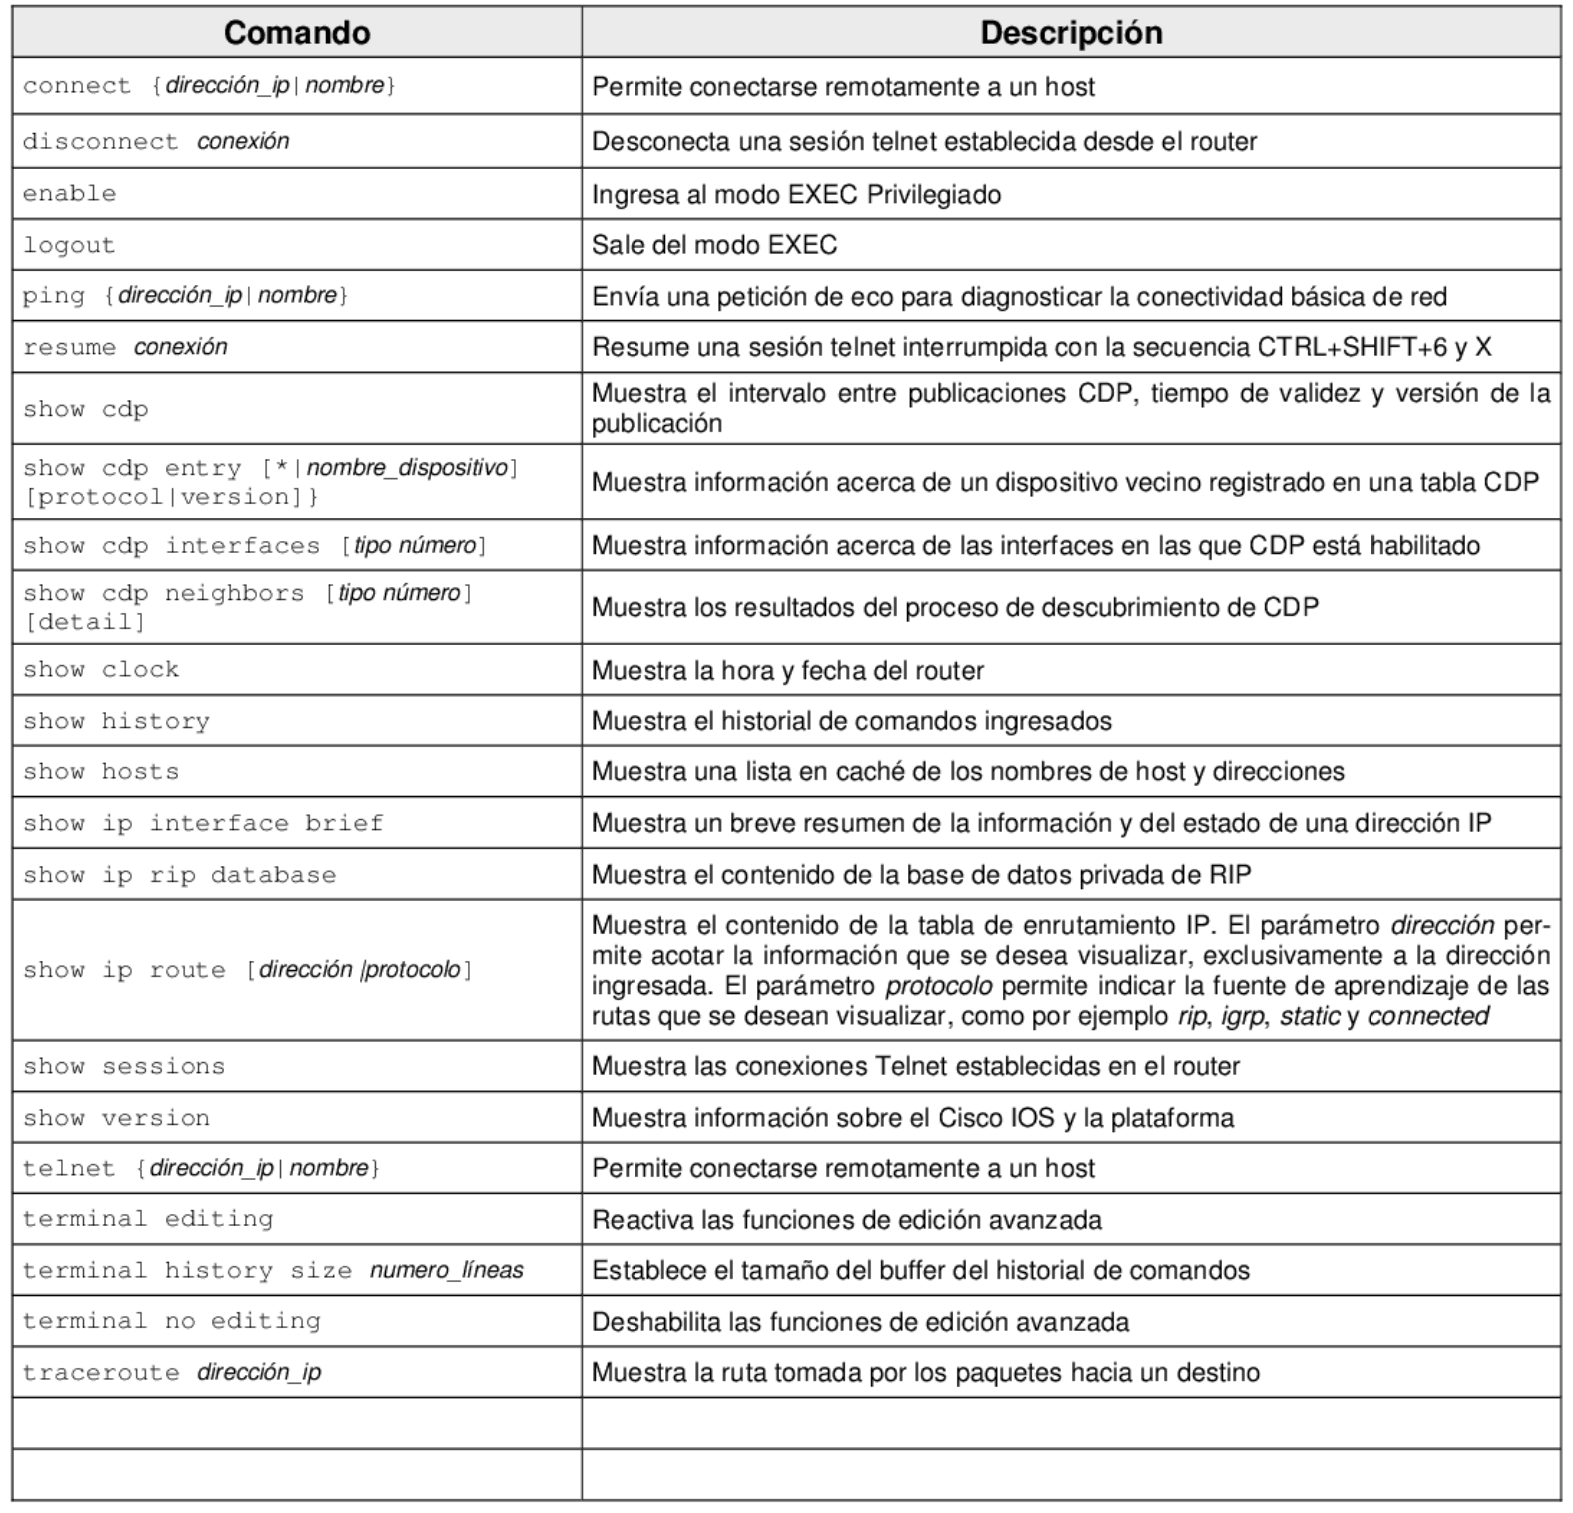
\includegraphics[scale=1]{Imagenes/router.png}
\end{center}

\begin{thebibliography}{9}
\bibitem{switches} 
Lorena Fernández.\href{https://www.redeszone.net/tutoriales/redes-cable/switch-gestionable-vs-no-gestionable-cual-elegir/}{https://www.redeszone.net/tutoriales/redes-cable/switch-gestionable-vs-no-gestionable-cual-elegir/} 4 de Julio, 2020

\bibitem{switches2} 
Gary McCauley. \href{https://www.fieldengineer.com/blogs/network-switch-managed-vs-unmanaged}{https://www.fieldengineer.com/blogs/network-switch-managed-vs-unmanaged} 1 de Julio, 2019

\bibitem{protos} 
Best Routing Protocol for a Bank \href{https://thwack.solarwinds.com/t5/General-Network-Discussions/Best-Routing-Protocol-for-a-Bank/m-p/366157}{https://thwack.solarwinds.com/t5/General-Network-Discussions/Best-Routing-Protocol-for-a-Bank/m-p/366157} 5 de Septiembre, 2012

\bibitem{protos2} 
Best Routing Protocol for a Bank \href{https://community.spiceworks.com/topic/223554-best-routing-protocol-for-a-bank}{https://community.spiceworks.com/topic/223554-best-routing-protocol-for-a-bank} 9 de Mayo, 2012

\bibitem{routing} 
\href{https://community.fs.com/blog/eigrp-vs-ospf-differences.html}{https://community.fs.com/blog/eigrp-vs-ospf-differences.html} 1 de Agosto, 2018.

\bibitem{routing2} 
SearchNetworking Staff \href{https://www.computerweekly.com/news/2240102196/Static-routing-for-Cisco-users-Day-Two-The-good-and-bad-of-static-routing}{https://www.computerweekly.com/news/2240102196/Static-routing-for-Cisco-users-Day-Two-The-good-and-bad-of-static-routing} 26 de Noviembre, 2006.

\bibitem{routing3}
What is Administrative Distance. \href{https://www.omnisecu.com/cisco-certified-network-associate-ccna/what-is-administrative-distance.php}{https://www.omnisecu.com/cisco-certified-network-associate-ccna/what-is-administrative-distance.php}

\bibitem{routing4}
Huawei NE20E-S V800R010C10SPC500 
\href{https://support.huawei.com/enterprise/en/doc/EDOC1100055120/8641f8b0/routing-protocol-and-route-priority}{https://support.huawei.com/enterprise/en/doc/EDOC1100055120/8641f8b0/routing-protocol-and-route-priority}

\bibitem{routing5}
What is Administrative Distance? Cisco \href{https://www.cisco.com/c/en/us/support/docs/ip/border-gateway-protocol-bgp/15986-admin-distance.html}{https://www.cisco.com/c/en/us/support/docs/ip/border-gateway-protocol-bgp/15986-admin-distance.html} 3 de Abril, 2020.

\bibitem{routing6}
Static and dynamic routing on same router. Cisco \href{https://community.cisco.com/t5/routing/static-and-dynamic-routing-on-same-router/td-p/3712613}{https://community.cisco.com/t5/routing/static-and-dynamic-routing-on-same-router/td-p/3712613} 24 de Septiembre, 2018.


\bibitem{routing7}
Can more than one protocol be run at the same time on a router? \href{https://community.cisco.com/t5/switching/can-more-than-one-protocol-be-run-at-the-same-time-on-a-router/td-p/2234948}{https://community.cisco.com/t5/switching/can-more-than-one-protocol-be-run-at-the-same-time-on-a-router/td-p/2234948} 5 de Agosto, 2013.

\bibitem{switch}
Ethernet Switches by Joann Zimmerman, Charles E. Spurgeon \href{https://www.oreilly.com/library/view/ethernet-switches/9781449367299/ch01.html}{https://www.oreilly.com/library/view/ethernet-switches/9781449367299/ch01.html}

\bibitem{switch2}
Ron Trunk, Respuesta en StackOverflow \href{https://networkengineering.stackexchange.com/questions/62568/using-different-speed-in-switch-ports}{https://networkengineering.stackexchange.com/questions/62568/using-different-speed-in-switch-ports}

\bibitem{g4g}
Cisco Switch Configuration basic commands \href{https://www.geeksforgeeks.org/cisco-switch-configuration-basic-commands/}{https://www.geeksforgeeks.org/cisco-switch-configuration-basic-commands/}


\end{thebibliography}
